%\documentclass{article}
\documentclass[a4paper,zihao=-4,UTF8]{ctexart}
\usepackage{xeCJK}
\usepackage{graphicx}  % 显示图片的
\usepackage{indentfirst}  % 可以设置首行缩进的
\usepackage{geometry} % 设置页边距
\usepackage{amsmath} % 公式对齐
 \usepackage{float} % 确保插入的图片就在固定的位置
\usepackage{titlesec} % 整体设置字号

\setlength{\parindent}{2em} %2em代表首行缩进两个字符
\geometry{a4paper,scale=0.83} % 设置页边距
\setCJKmainfont{简宋} % 将SimSun替换为你系统中的中文字体
\linespread{1.5}%修改行距

% 设置 section 和 subsection 的字体大小
\titleformat*{\section}{\fontsize{16}{19.2}\selectfont\bfseries}
\titleformat*{\subsection}{\fontsize{14}{17.5}\selectfont\bfseries}


\begin{document}
	\title{家庭暴力的经济学模型}
	\author{杨景媛}
	\date{2024年2月4日} 
	\maketitle

%	\fontsize{14pt}{17.5pt}\selectfont % 设置正文字号和行距


	\section*{模型的基本设定}	
	考虑一对夫妇,包含一个男性$m$和一个女性$f$,他们在劳动力市场上获得的工资分别为$w_m$与$w_f$。在考虑婚姻的收益时,可以从两方面讨论,一方面是结婚带来的规模效应,使得家庭收入大于男性与女性单身收入之和;另一方面,婚姻独有的产出品也给夫妻双方提供了效用。根据Becker(1973)当中提出的理论,共同生育的后代是婚姻区别于其他家庭关系的重要体现。因此在这个模型当中我们也考虑了子女给夫妻带来的效应。给出家庭的整体效用函数为:
	\begin{equation}
		U = (1+\alpha)(w_m+w_f+b\varphi)
	\end{equation}
	其中$\alpha$表示婚姻的规模效应,$b \in \{0,1\}$表示家庭是否有孩子,$\varphi$表示生育后代带来的净效应。
	
	经过家庭内部的议价之后,妻子和丈夫会共同分享家庭整体效用,在这里我们假定双方的初始议价权是平等的,因此,丈夫和妻子通过婚姻所能得到的效用如下:
	\begin{equation}
		\left\{
		\begin{array}{lr}
			u_m = \frac{1}{2}(1+\alpha)(w_m+w_f+b\varphi) \\
			u_f =  \frac{1}{2}(1+\alpha)(w_m+w_f+b\varphi)
		\end{array}
		\right.
	\end{equation}
	
	
	\section*{已婚未育的情况下,家暴行为的成本收益}
	
	首先我们考虑一对单身男女(见图1),此时这对单身男女的效用可能性边界(utility-possibility frontier)为图中的$AB$曲线,假定二人的初始状态为$e_0(u_{f0},u_{m0})$,当二人结婚后,由于规模效应,家庭的总收益大于二人单身时的工资收益之和,因此家庭的总效用为(图1 中用$CD$曲线表示):
	\begin{equation}
		U_0 = (1+\alpha)(w_m+w_f)
	\end{equation}
	由于前文我们设定双方的初始议价权是平等的,此时丈夫与妻子的效用水平分别为(图中均衡点为$e_0'$):
	\begin{equation}
		\left\{
		\begin{array}{lr}
			u_m^{A_0} = \frac{1}{2}(1+\alpha)(w_m+w_f) \\
			u_f^{A_0} =  \frac{1}{2}(1+\alpha)(w_m+w_f)
		\end{array}
		\right.
	\end{equation}
	在已婚未育的婚姻当中,存在的outside option为离婚(恢复单身),在这种情况下,夫妻双方的outside option分别为:
	\begin{equation}
		\left\{
		\begin{array}{lr}
			\bar{u}_{m0} = w_m \\
			\bar{u}_{f0}= w_f
		\end{array}
		\right.
	\end{equation}
	上述假设基本和实际相符,我们可以在日常生活中观察到,已婚未育的夫妻离婚后在婚姻市场上的定位基本等同于未婚个体,因此我们假设已婚未育的夫妻在婚姻中存在的outside option就是单身状态时的效用。
	
	接下来,我们在模型当中引入家暴。在引入家暴的时候,我们需要两个基本的假定:
	\begin{itemize}
		\item 首先,丈夫进行家暴的直接原因是通过暴力提高自身在家庭当中的议价能力,以期望能分配到更多的婚姻产出,因此,本文在这里设定$T$作为家庭暴力带来的婚姻产出的内部转移。
		\item 其次,家庭暴力是存在成本的。家暴的成本可以通过多个角度来理解:例如家暴降低了女性在婚姻当中的生产积极性,使得家庭总产出降低;又或者家暴给女性身体造成了伤害,从而使得家庭总产出降低。此外,如果政府对家暴行为进行严格管制,例如在发现家暴的时候,给予严厉的处罚,类似的法律制度会极大的增大家庭暴力的成本。在本文中,为了使模型简单明了,我们假设家庭暴力的成本为常数$C$。因此,当存在家庭暴力时,家庭的效用可能性边界从$CD$内推至$C'D'$,均衡点也移动至$e_0''$
	\end{itemize}
	当存在家庭暴力时,此时家庭总效用为:
		\begin{equation}
		U_0^{A_1} = (1+\alpha)(w_m+w_f)-C
	\end{equation}
	此时,夫妻双方的效用为:
	\begin{equation}
	\left\{
	\begin{array}{lr}
		u_m^{A_1} = \frac{1}{2}[(1+\alpha)(w_m+w_f)-C]+T \\
		u_f^{A_1} =  \frac{1}{2}[(1+\alpha)(w_m+w_f)-C]-T 
	\end{array}
	\right.
\end{equation}

\begin{figure}[htbp]
	\centering
	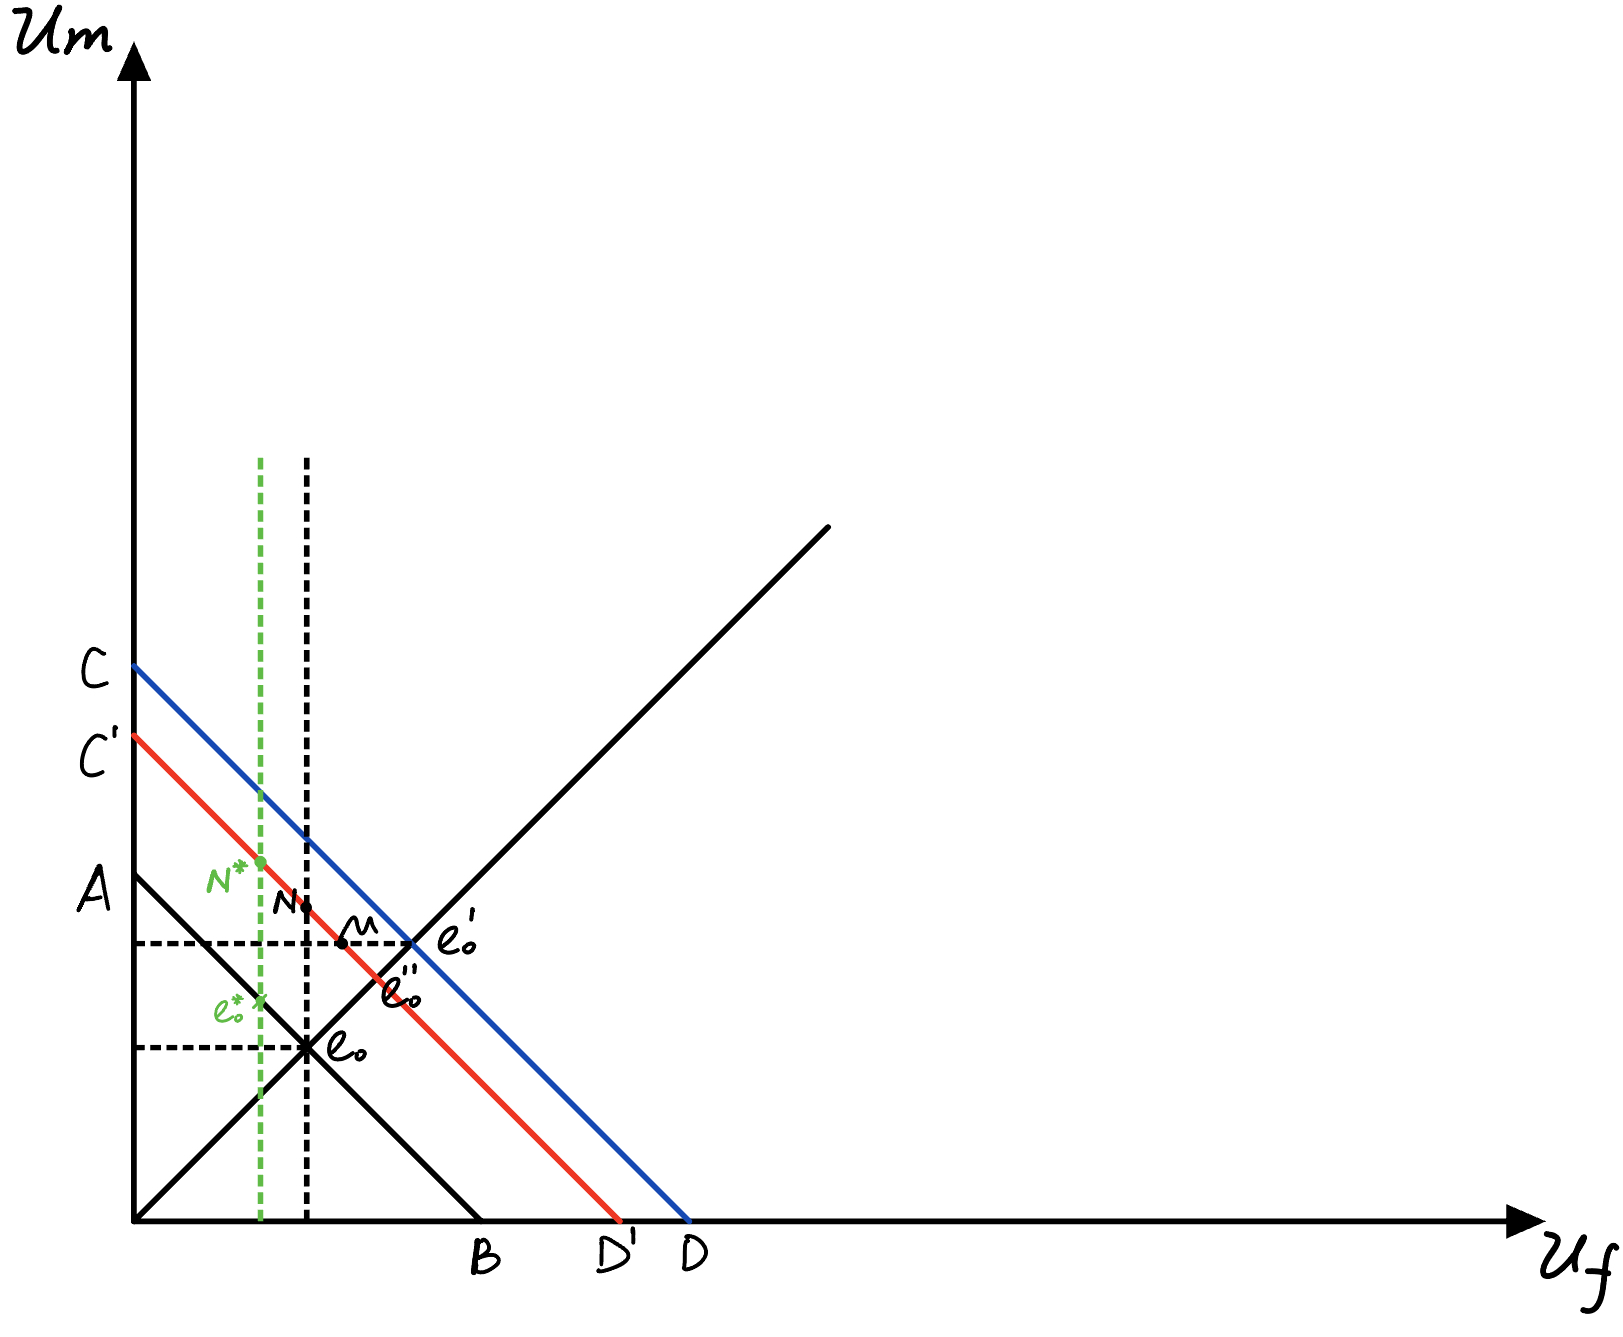
\includegraphics[width=80mm]{pic/figure1.png}
	\caption{已婚未育时家暴的成本收益}
\end{figure}

	\subsection*{家暴存在的条件}
	丈夫选择家暴的条件是通过家暴获取的效用转移大于家暴前获得的效用。如图 1所示,当家暴发生后均衡点在为$e_0''M$上时,家暴不会发生,因为此时丈夫的效用是低于家暴前获得的效用的,基于家暴的成本与收益,我们可以计算得到在家暴发生临界点,家暴成本$C$与家暴收到效用转移$T$之间的关系::
	首先,家暴发生的条件是$u_{m0}^{A_1}>u_{m0}^{A_0}$,即:
	\begin{equation}
		\begin{aligned}
			\frac{1}{2}[(1+\alpha)(w_m+w_f)-C]+T &> \frac{1}{2}(1+\alpha)(w_m+w_f) \\
			C &< 2T
		\end{aligned}
	\end{equation}
	因此,当家暴的成本较高,通过家暴丈夫获取的效用转移又有限时,家暴便不会发生。政府可以通过提高家暴的成本来减少家暴的发生,除了对家暴者施加惩罚以外(例如拘留等),也可以通过减少家庭的共同产出(例如罚款等)来降低家暴的可能性。

	\subsection*{丈夫通过家暴所能攫取的最大效用}
	丈夫通过家暴可以攫取的效用并非是无限的,当妻子被家暴后得到的效用少于outside option时,妻子会选择退出婚姻,因此,我们可以在$u_f^{A_1}=	\bar{u}_{f0}$的零界点上计算得到丈夫通过家暴可以攫取的最大效用。
	\begin{equation}
		\begin{aligned}
			u_{f0}^{A_1}  &=	\bar{u}_{f0}  \\
			\frac{1}{2}[(1+\alpha)(w_m+w_f)-C]-T &= w_f  \\
			T_{0,max}&=\frac{1}{2}(1+\alpha)w_m+\frac{1}{2}(\alpha -1) w_f-\frac{1}{2}C
		\end{aligned}
	\end{equation}
	
体现在图 1 中,当丈夫通过家暴得到了最大的效用转移时,此时的均衡点为$N(w_f,(1+\alpha)w_m+\alpha w_f-C)$。家暴所能带来的效用转移$T \in [\frac{1}{2}C, \frac{1}{2}(1+\alpha)w_m+\frac{1}{2}(\alpha -1) w_f-\frac{1}{2}C]$,当家暴带来的效用$T$小于这个区间时,家暴带来的收益不足以弥补家暴带来的损失,此时家暴不会发生;而当家暴带来的效用$T$大于这个区间时,妻子会因为婚内效用差于outside option而选择退出婚姻。因此,均衡点可能的位置在$MN$上。

此外,回到模型的最初设定,我们假定了一对婚前收入大致相同的单身男女,其婚前均衡点为$e_0$,如果我们在同样的效用可能性边界$AB$曲线上移动初始点到$e_0^*$,这意味着婚前丈夫的收入较多,而妻子的收入较少,那么在夫妻双方面临的outside option当中,妻子会面临一个更差的外部选择,因此她会家庭暴力的忍耐度也会更高,丈夫通过家庭暴力所能攫取的效用就从$e_0''N$增加到了$e_0''N^*$。模型的这一设定和现实也具有很好的符合度,在夫妻双方收入差异较大的情况下,丈夫在婚后发生家庭暴力的概率会更高(在实证中我需要验证这一点)。

	\section*{已婚已育的情况下,家暴行为的成本收益}	
	在已婚已育$(b=1)$的情况下,家庭的总效用函数为:
	\begin{equation}
		U_1=(1=\alpha)(w_m+w_f+\varphi)
	\end{equation}
	当不存在家暴时,丈夫与妻子的效用水平分别为:
		\begin{equation}
		\left\{
		\begin{array}{lr}
			u_m = \frac{1}{2}(1+\alpha)(w_m+w_f+\varphi) \\
			u_f =  \frac{1}{2}(1+\alpha)(w_m+w_f+\varphi)
		\end{array}
		\right.
	\end{equation}
	当存在家庭暴力时,家庭的总效用函数为:
	\begin{equation}
		U_1^{A_1}=(1+\alpha)(w_m+w_f+\varphi)-C
	\end{equation}
	在分析已婚未育的情况时,我们假定结婚并不会影响夫妻双方的outside option,但对于已婚已育的夫妻而言,生育将会在很大程度上影响到二者的outside option,且这一影响对于夫妻双方而言很可能有很大的不同。因此在已婚已育的情况下,我们将分两个角度讨论家庭暴力的成本收益问题。在第一个角度中,我们假设生育对于夫妻双方outside option的影响程度是相同的,生育的收益和成本在男女双方当中均分;而第二个角度则更贴合实际,女性将承担更多的生育成本,在这种情况下,我们会发现丈夫的家暴概率和通过家暴攫取的效用会更多。

	\subsection*{假设生育对夫妻双方outside option的影响程度是相同的}
	在已婚已育的家庭中(见图 2),家庭的效用可能性边界用$EF$曲线来表示,当存在家庭暴力时,家庭的效用可能性边界内推至$E'F'$,此时均衡点为$e^{''}_1$。同时,已婚已育的家庭中,在生育不影响女性outside option的情况下,夫妻双方面临的outside option为点$e_1$:
	\begin{equation}
	\left\{
	\begin{array}{lr}
		\bar{u}_{m1} = w_m +\frac{1}{2} \varphi \\
		\bar{u}_{f1 }= w_f+\frac{1}{2} \varphi 
	\end{array}
	\right.
	\end{equation}
	\begin{figure}[H]
		\centering
		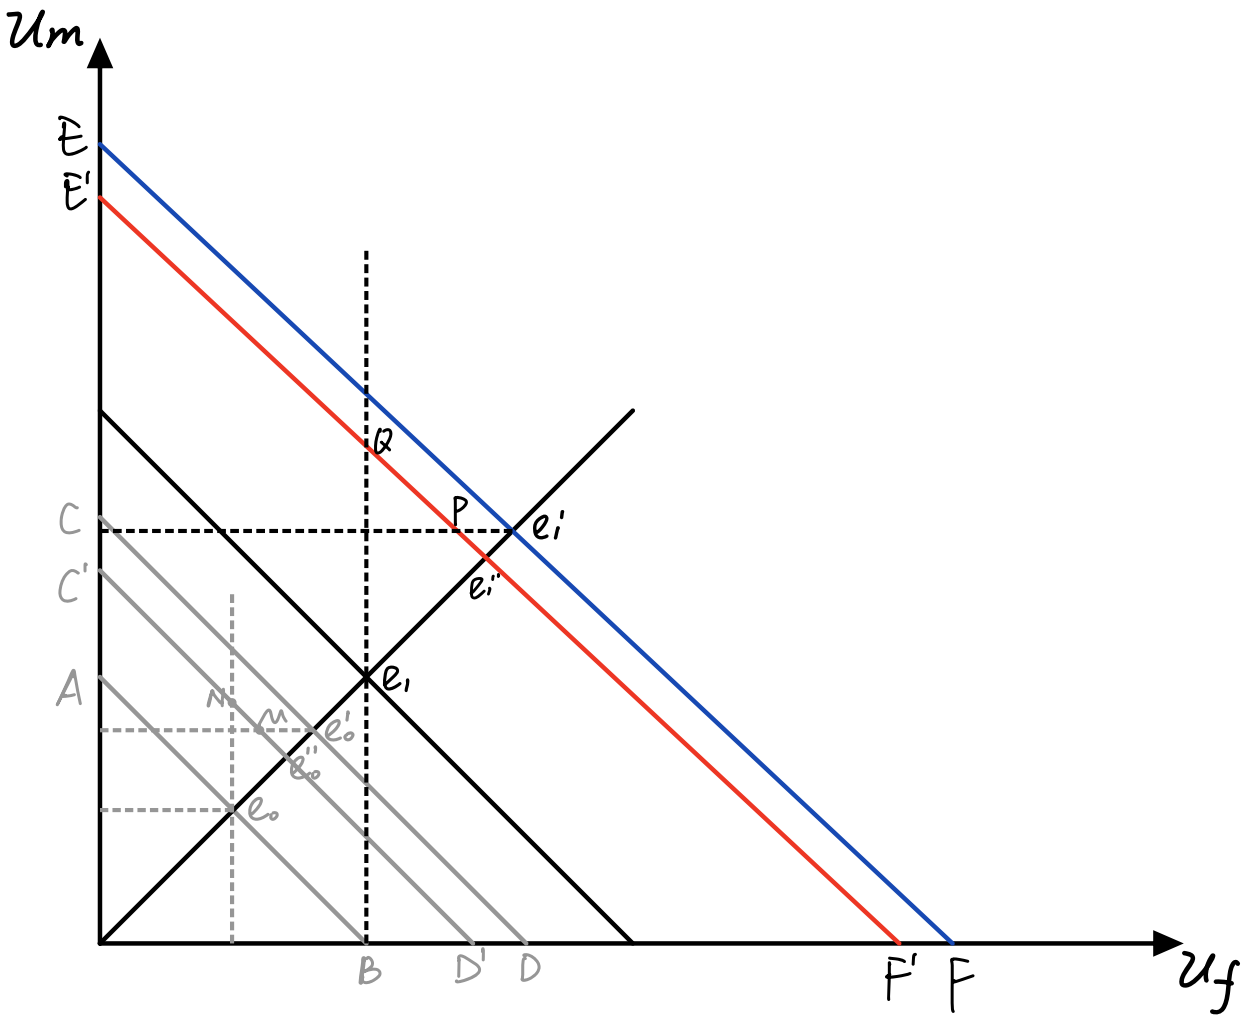
\includegraphics[width=80mm]{pic/figure2.png}
		\caption{\centering}{已婚已育时家庭暴力的成本收益\\(假设生育对夫妻双方outside option的影响是相同的)}
	\end{figure}
	当存在家庭暴力时,夫妻双方效用为点$e^{''}_1$(即离婚后均分生育带来的净收益):
	\begin{equation}
	\left\{
	\begin{array}{lr}
		u_m^{A_1} = \frac{1}{2}[(1+\alpha)(w_m+w_f+\varphi)-C]+T \\
		u_f^{A_1} =  \frac{1}{2}[(1+\alpha)(w_m+w_f+\varphi)-C]-T 
	\end{array}
	\right.
\end{equation}
	同样的,我们可以计算得到发生家暴的临界条件:$u_{m1}^{A_1}>u_{m1}^{A_0}$,即当$C>2T$时,不会发生家暴,体现在图中即为均衡点在$e^{''}_1P$上:
	此外,我们也可以计算得到丈夫能够通过家暴攫取到的最大效用:
	\begin{equation}
	\begin{aligned}
		u_{f1}^{A_1}  &=	\bar{u}_{f1}  \\
		\frac{1}{2}[(1+\alpha)(w_m+w_f+\varphi)-C]-T &= w_f+\frac{1}{2}\varphi \\
		T_{1,max}&=\frac{1}{2}(1+\alpha)w_m+\frac{1}{2}\alpha w_f+\frac{1}{2}\alpha \varphi-\frac{1}{2}C
	\end{aligned}
\end{equation}

相较于未婚未育的情况,已婚已育的情形中,丈夫能够通过家暴攫取更多的效用,多出来的这一部分为$\frac{1}{2}\alpha \varphi$,正如Becker(1973)当中所述,共同产生的后代是婚姻产出当中最重要的部分,因为婚姻所带来的其他好处:例如规模效应、照料、关爱等都可以通过其他家庭关系带来,但后代只能通过婚姻关系产出。此外,$\frac{1}{2}\alpha \varphi$也表明,婚姻当中二人的合作关系有效的降低了育儿成本,换句话说,婚姻关系中因为夫妻双方可以共同抚养后代,这使得生育带来的效用被放大了。
	
	
	\subsection*{允许生育对夫妻双方的outside option有不同程度的影响}
	在上一小节中,我们假定生育对夫妻双方outside option的影响是相同的,当婚姻关系破裂后,生育后代的净效用会被双方平分。而在这一节中,我们将放松这一假定,因为在现实当中,妻子往往承担了更多的生育成本(例如因为生育而脱离就业市场、因为生育造成的身体损伤等等),而在离婚后,无论孩子的抚养权归哪一方,丈夫实际上都享有了生育后代更多的净收益(这一部分还需要更多的举例,随父姓在大多数人眼里并不是很大的利益)。此外,已婚已育后的夫妻在婚姻关系破裂后,其在婚姻市场上和单身人士(或已婚未育的离婚人士)处在不同的匹配地位。尤其是生育后的女性在婚姻市场上似乎更加不受欢迎(这一点我不确定,需要再核实)。因此从多个方面来分析,已婚已育夫妻的outside option中,女性会面临一个更差的选择:
	\begin{equation}
		\begin{cases}
			\bar{u}_{m1}^* = w_m+\gamma \varphi \\
			\bar{u}_{f1}^* = w_f+(1-\gamma)\varphi
		\end{cases} , \quad \gamma > \frac{1}{2}
	\end{equation}
	
	\begin{figure}[H]
		\centering
		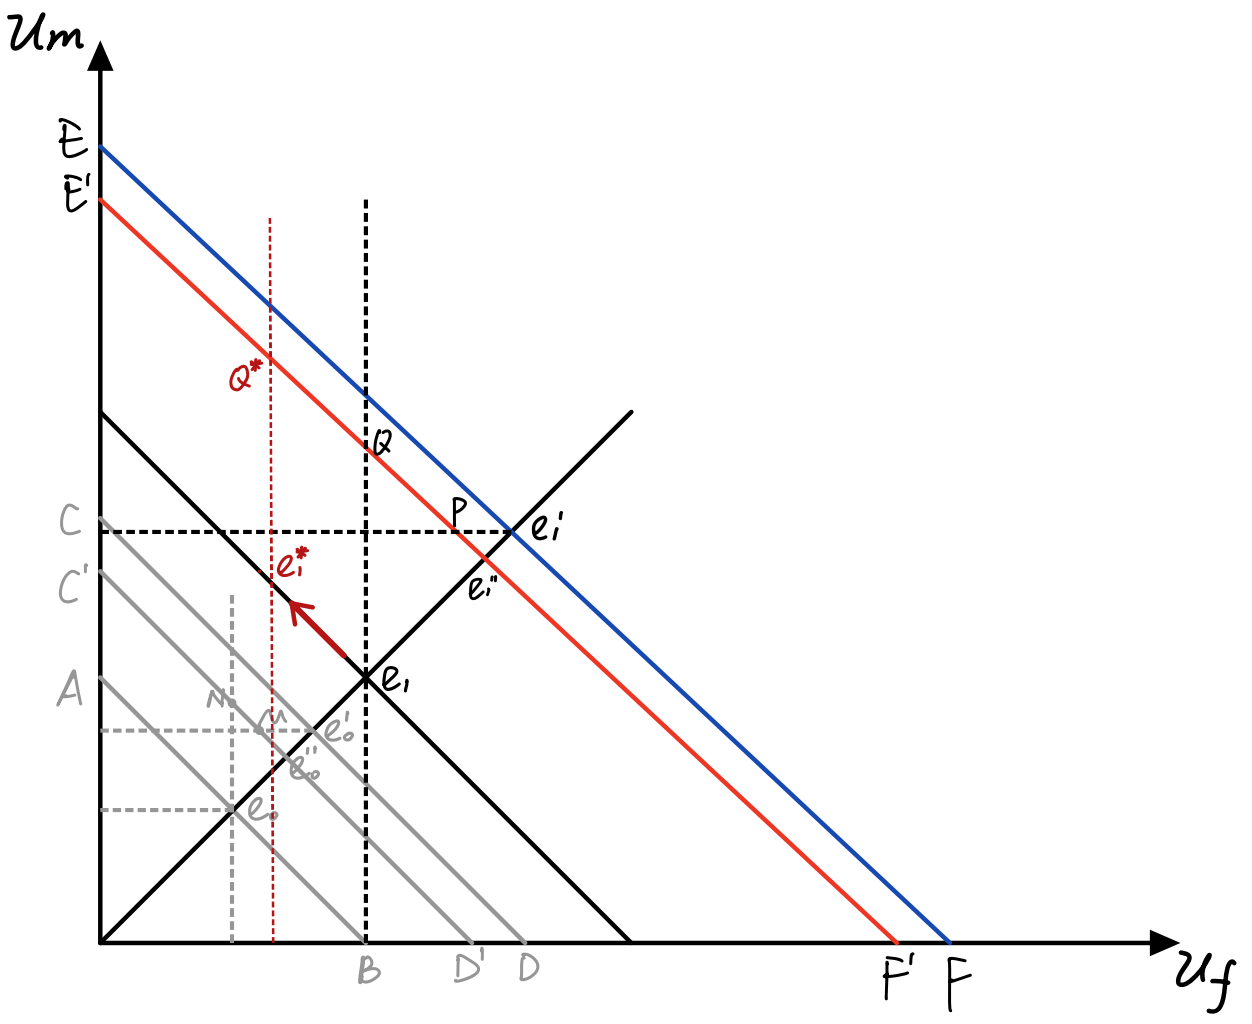
\includegraphics[width=80mm]{pic/figure3.png}
		\caption{\centering}{已婚已育时家庭暴力的成本收益\\(假设生育影响对夫妻双方outside option的影响程度是不同的)}
	\end{figure}
	
	具体在图中(见图 3),即为outside option从$e_1$移动到$e_1^*$。由于妻子outside option的恶化使得男性可以通过家暴攫取的效用区间变大,因此此时的家暴可能性区间从$e''_1Q$延长到$e''_1Q^*$。值得注意的是,如果生育对女性outside option的改变足够大,使得$e_1^*$无限接近与$y$轴,这可能使得女性无法离开家暴环境。类似的情形在现实中并非无迹可寻,例如很多已婚女性会为了孩子选择对丈夫的家暴行为默默忍受,而不离婚或寻求外界帮助。








	

\end{document}